\documentclass{article}
\usepackage[utf8]{inputenc}
\usepackage[hidelinks]{hyperref}
\usepackage{amsmath}
\usepackage[noabbrev, capitalise]{cleveref}
\usepackage{amssymb}
\usepackage{graphicx}
\usepackage{float}
\usepackage{subfig}
\usepackage{booktabs}
\usepackage[parfill]{parskip}

\usepackage[sorting=none]{biblatex}
\addbibresource{report_1.bib}

\usepackage{titling}
\setlength{\droptitle}{-3cm}

\title{COMP6247 Lab 1: Recursive Least Squares}
\author{Wei Chien Teoh (Eugene)\\\bigskip \href{mailto:wct1c16@soton.ac.uk}{wct1c16@soton.ac.uk}}
\date{22 February 2021}

\begin{document}

\maketitle

\section{Introduction}

This report presents to findings and results for Lab 1 of COMP6247 of University of Southampton \cite{lab1}. The code implementation is stored in a Github repository \cite{github}.

\section{Task 1}

The task 1 of the exercise is to implement a simple linear regression on synthetic data solved with three different methods, namely: (i) closed form (pseudo-inverse); (ii) gradient descent (GD); (iii) stochastic gradient descent (SGD). The synthetic data generated involves a design matrix $X \in \mathbb{R}^{N \times p}$ and a set of weights $w_* \in \mathbb{R}^p$. In this example, $N$ (number of sample) and $p$ (number of features) are set to 500 and 30 respectively. The data are generated from a gaussian distribution $X, w_* \sim \mathcal{N}(0.5, 1)$ using Numpy. The target data $y$ is defined as the product $Xw_*$ added with noise also sampled from a gaussian distribution $\mathcal{N}(0, 1)$.

% TODO: PCA to show plots

\cref{fig:lr_closed} shows the predicted results against the true values of targets and weights. Although the variance of the plots are large, there exist a linear relationship between true values and the prediction. This means that the closed form solution successfully provided a solution for the linear regression. The result plots for GD and SGD are very similar to that of \cref{fig:lr_closed}, hence they will be excluded in this report.

\begin{figure}[h!]
    \centering
    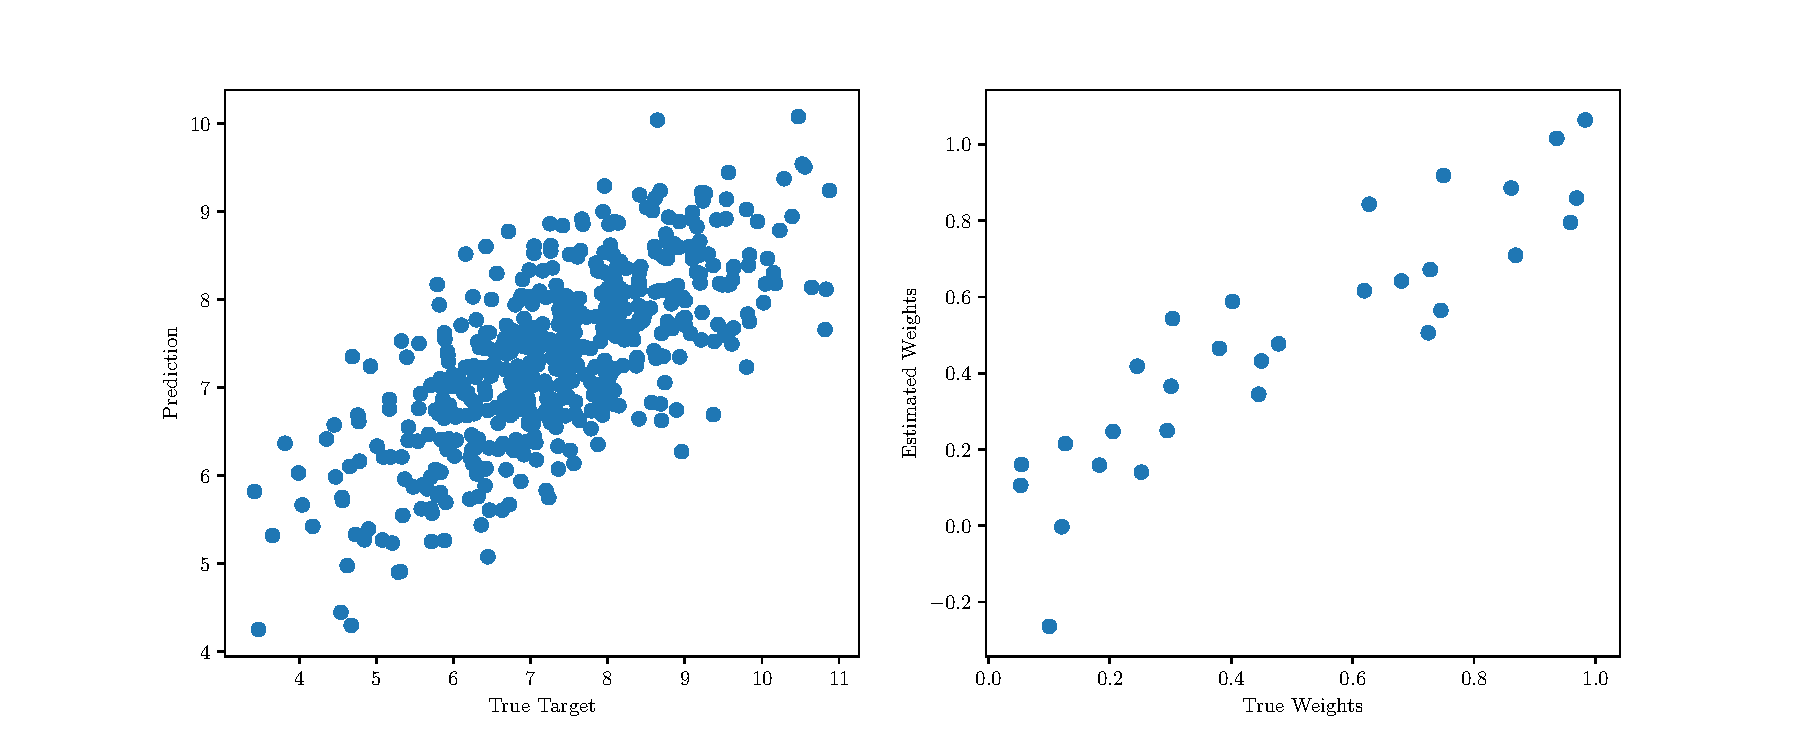
\includegraphics[width=\textwidth]{Figures/closed.pdf}
    \caption{Results of Linear Regression estimated with closed form. (Left) true value of target against prediction. (Right) true values of weights against estimated weights.}
    \label{fig:lr_closed}
\end{figure}

\cref{tab:task1_corr} shows the pearson correlation of the above three methods of estimating the solution for linear regression. All three methods show promising and very close results. Thus, it can be concluded that all three methods successfully estimated the linear regression. Out of the three, the closed form solution performed the best.

The loss function of linear regression is convex, hence there exist a closed form solution. However, if the number of features $p$ is large, the pseudo-inverse may be expensive to compute. The time complexity of matrix inversion using the Gaussian elimination is $\mathcal{O}(n^3)$, hence it does not scale with larger matrices.

\begin{table}[h!]
    \centering
    \caption{Pearson correlation of predicted values against ground truth.}
    \label{tab:task1_corr}
    \begin{tabular}{lrr}
    \toprule
    {} &    Target &   Weights \\
    \midrule
    Ground Truth &  1.000000 &  1.000000 \\
    Closed Form  &  0.704550 &  0.901110 \\
    GD           &  0.704474 &  0.901734 \\
    SGD          &  0.695540 &  0.911628 \\
    \bottomrule
    \end{tabular}
\end{table}

\cref{fig:gd_training} shows the training error against the number of iterations for two variants of gradient descent, batch and stochastic. \cref{fig:gd} shows the batch gradient descent training with the learning rate set to $10^{-4}$ for 500 iterations. \cref{fig:sgd} shows the stochastic gradient descent training with learning rate set to 0.005 for 5000 iterations.

With batch gradient descent, it requires less iterations than stochastic gradient descent to achieve the convergence of the loss function. It also shows a smoother convergence with less fluctuation of error. However, as the number of data samples $N$ gets larger, the derivative of the loss function with respect to the weights, $\nabla_{\boldsymbol{w}} E$ will be more expensive to compute.

Stochastic gradient descent was proposed to provide a scalable solution with large $N$. \cref{fig:sgd} show the training error across the number of iterations. SGD provides similar performance to batch gradient descent, but with much more fluctuation. If the training is stopped at a training iteration with high fluctuation, it will cause the error at that iteration to be large. \cref{fig:sgd_noise} shows visual intuition of gradient descent updates close the convergence of loss function. The fluctuations of \cref{fig:sgd} are caused by oscillations between the valley of the convex loss function.

\begin{figure}[H]
    \subfloat[Batch Training]{\label{fig:gd}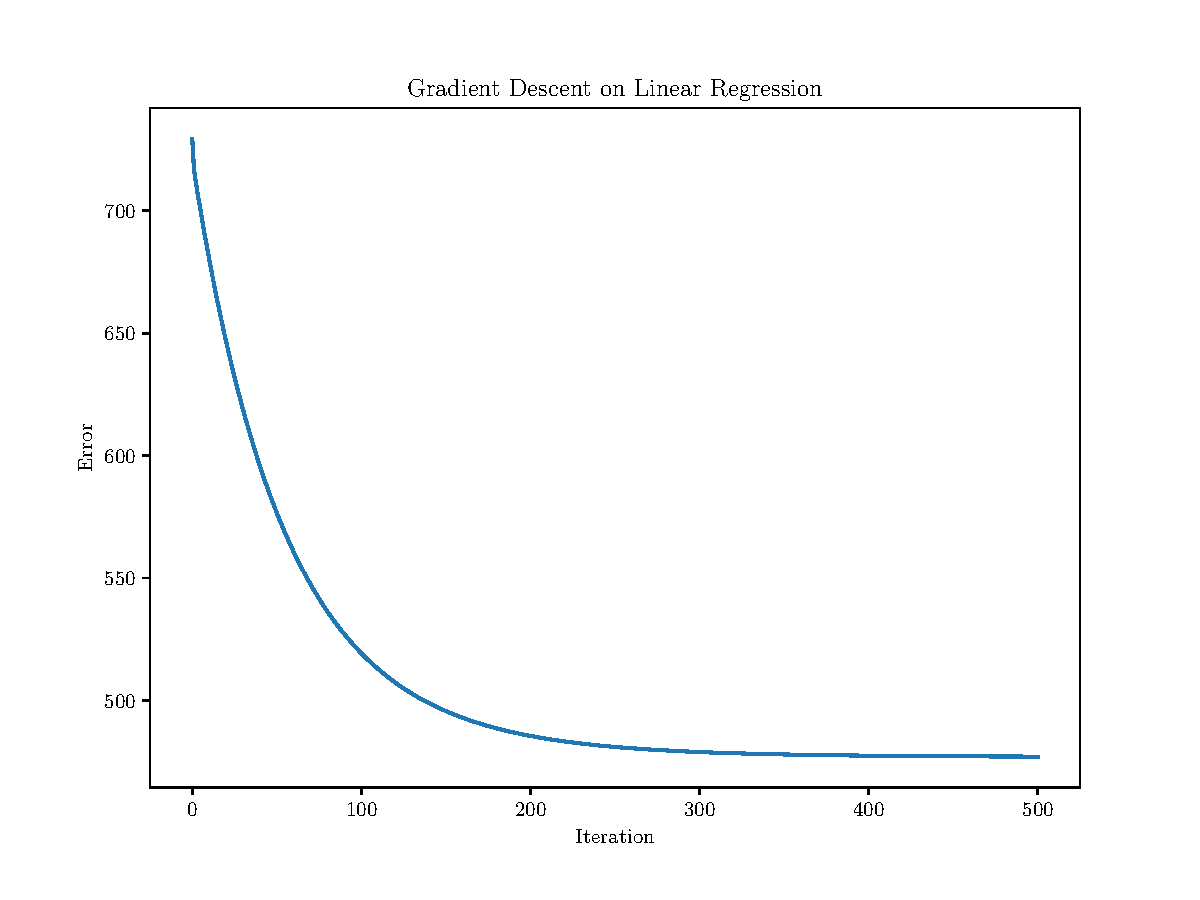
\includegraphics[width=0.5\textwidth]{Figures/gd_iterError.pdf}}
    \subfloat[Stochastic Training]{\label{fig:sgd}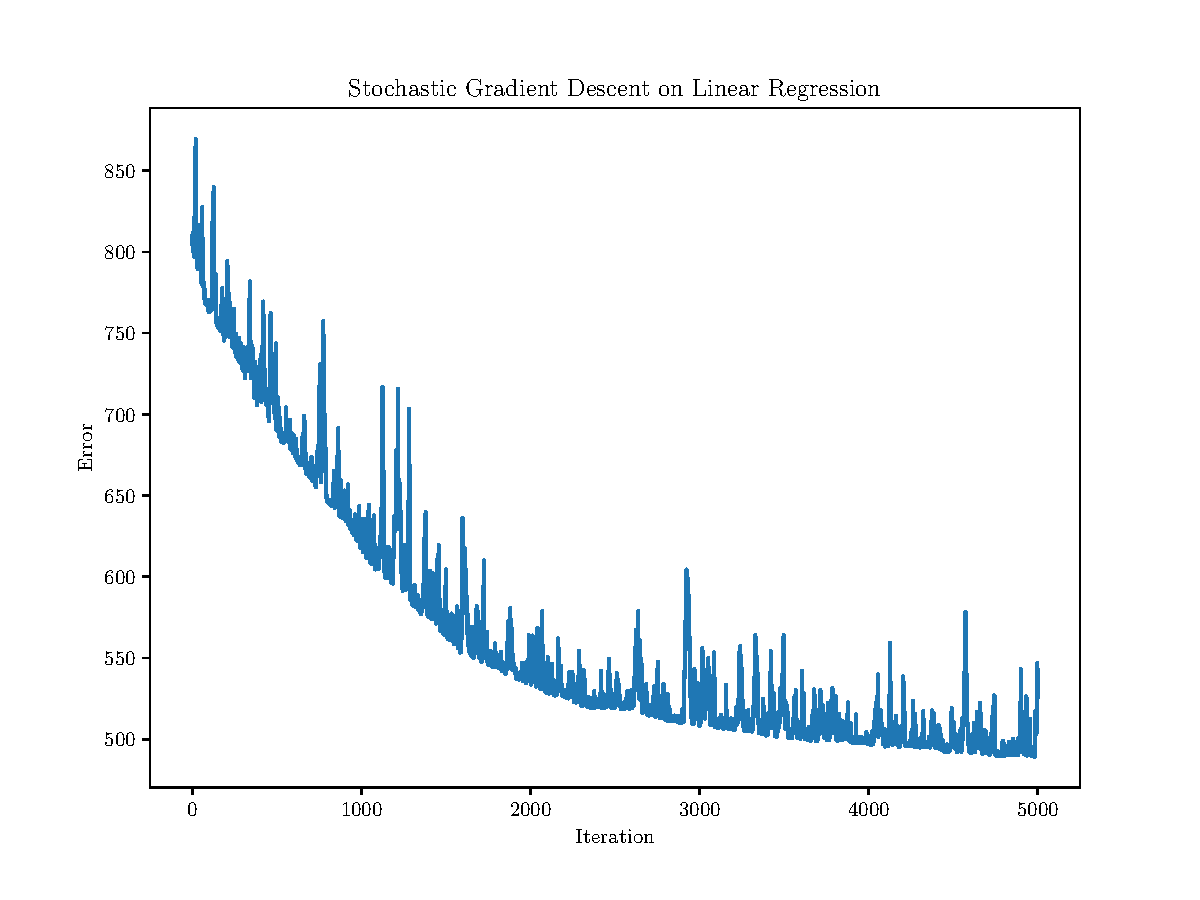
\includegraphics[width=0.5\textwidth]{Figures/sgd_iterError.pdf}}
    \caption{Gradient Descent Training of Linear Regression.}
    \label{fig:gd_training}
\end{figure}

\begin{figure}[H]
    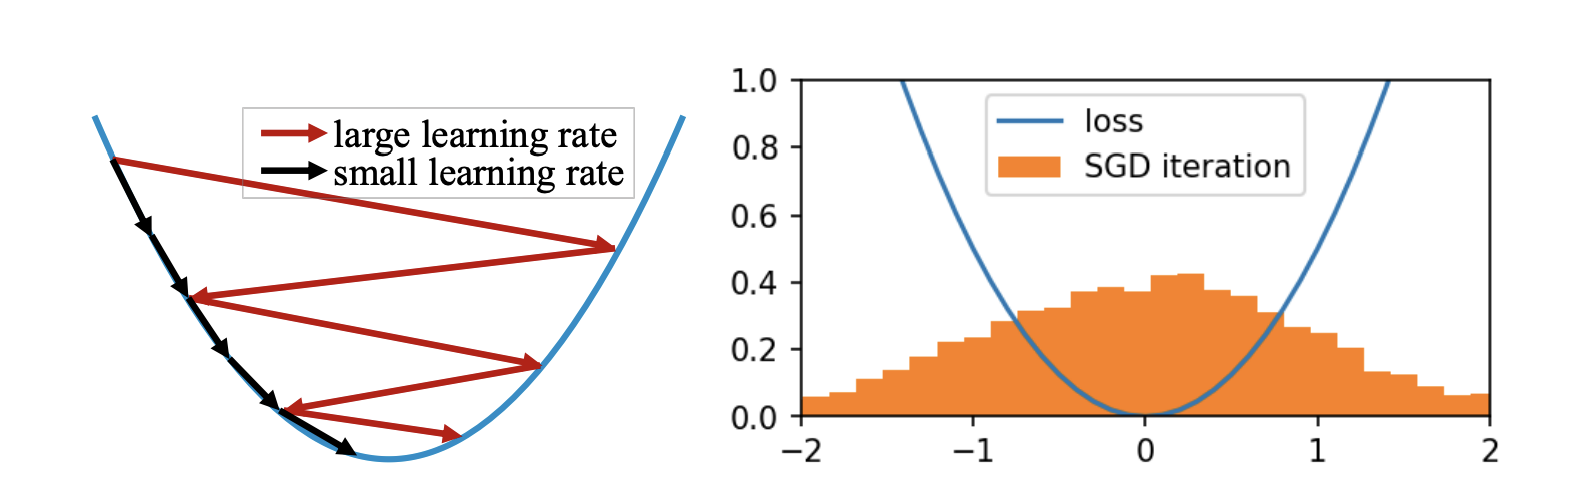
\includegraphics[width=\textwidth]{Figures/sgd_update.png} 
    \caption{(Left) Effects of magnitude of learning rate on gradient descent update. (Right) Distribution of SGD loss convergence. (Sourced from \cite{liu2021noise})}
    \label{fig:sgd_noise}
\end{figure}

% TODO: Introduce mini-batch gradient descent




\section{Task 2}

\section{Task 3}

\section{Task 4}

\printbibliography

\end{document}